\section{Logistics}
\label{sec:fdsp-tc-log}

%%%%%%%%%%%%%%%%%%%%%%%%%%%%
\subsection{Introduction}
\label{sec:fdsp-tc-log-intro}
The transportation of equipment and people underground is one of the more challenging aspects of the LBNF/DUNE endeavor. The access underground is via the mile long Ross shaft, which is now undergoing renovation. The shaft is outfitted with a single cage for people and materials and two skips which are needed for removing the rock underground. Planning the usage of the cage is one of the most important exercises in making LBNF/DUNE a success. Given the enormous cost of the conventional facilities (CF) contracts and the large cost of any inefficiencies in construction the overall coordinator of the Ross Shaft for LBNF/DUNE will be the CF Central Manager General Contractor (CMGC). Both LBNF and DUNE will also have a large number of contractors, institutions, and scientists who will need to bring equipment and materials underground. LBNF/DUNE will establish a logistics organization in South Dakota near SURF to facilitate the flow of material and people to the underground area. This organization will be responsible for receiving all goods for LBNF (except CF) and DUNE,
for coordinating the transport of this material underground with the CF-CMGC, and
for coordinating personnel usage of the Ross cage with the CF CMGC. 


%\begin{dunetable}
%[Logistics Specifications]
%{ll}
%{tab:table-Log-Req}
%{Table of logistics specifications.}
%Specifications &  \\ \toprowrule
%Material Handling & Comply with the SURF Material %Handling Specification \\ \colhline
%CMGS coordination & Provide CMGC with two-week notice %of shipments to SURF \\ \colhline
%Stage DUNE Shipments & Provide a one-month local %buffer of DUNE materials \\
%\colhline
%\dword{apa} Storage & Provide storage space for 150 %\dword{apa}s in a clean environment \\
%\colhline
%Inventory & Provide an inventory system accessible to %the collaboration \\
%\end{dunetable}
 %\fixme{Specifications table needs to be converted to official format}
 
 A high-level overview of the material flow to the Ross shaft is shown in Figure~\ref{fig:logistics-material-flow}. Freight is delivered to a central South Dakota Warehouse Facility (SDWF) with possible exception of the cryogenic equipment. 
 The materials are then transported in a "just--in--time" fashion to the Ross headframe where they are brought underground. For the detector the \dword{apa} electronics and photon detector components will also be shipped to the Integration Test Facility where they are assembled and then shipped back to SDWF.
 
\begin{dunefigure}[Material flow diagram for logistics ]{fig:logistics-material-flow}
  {Material Flow diagram for the LBNF/DUNE logistics.}
 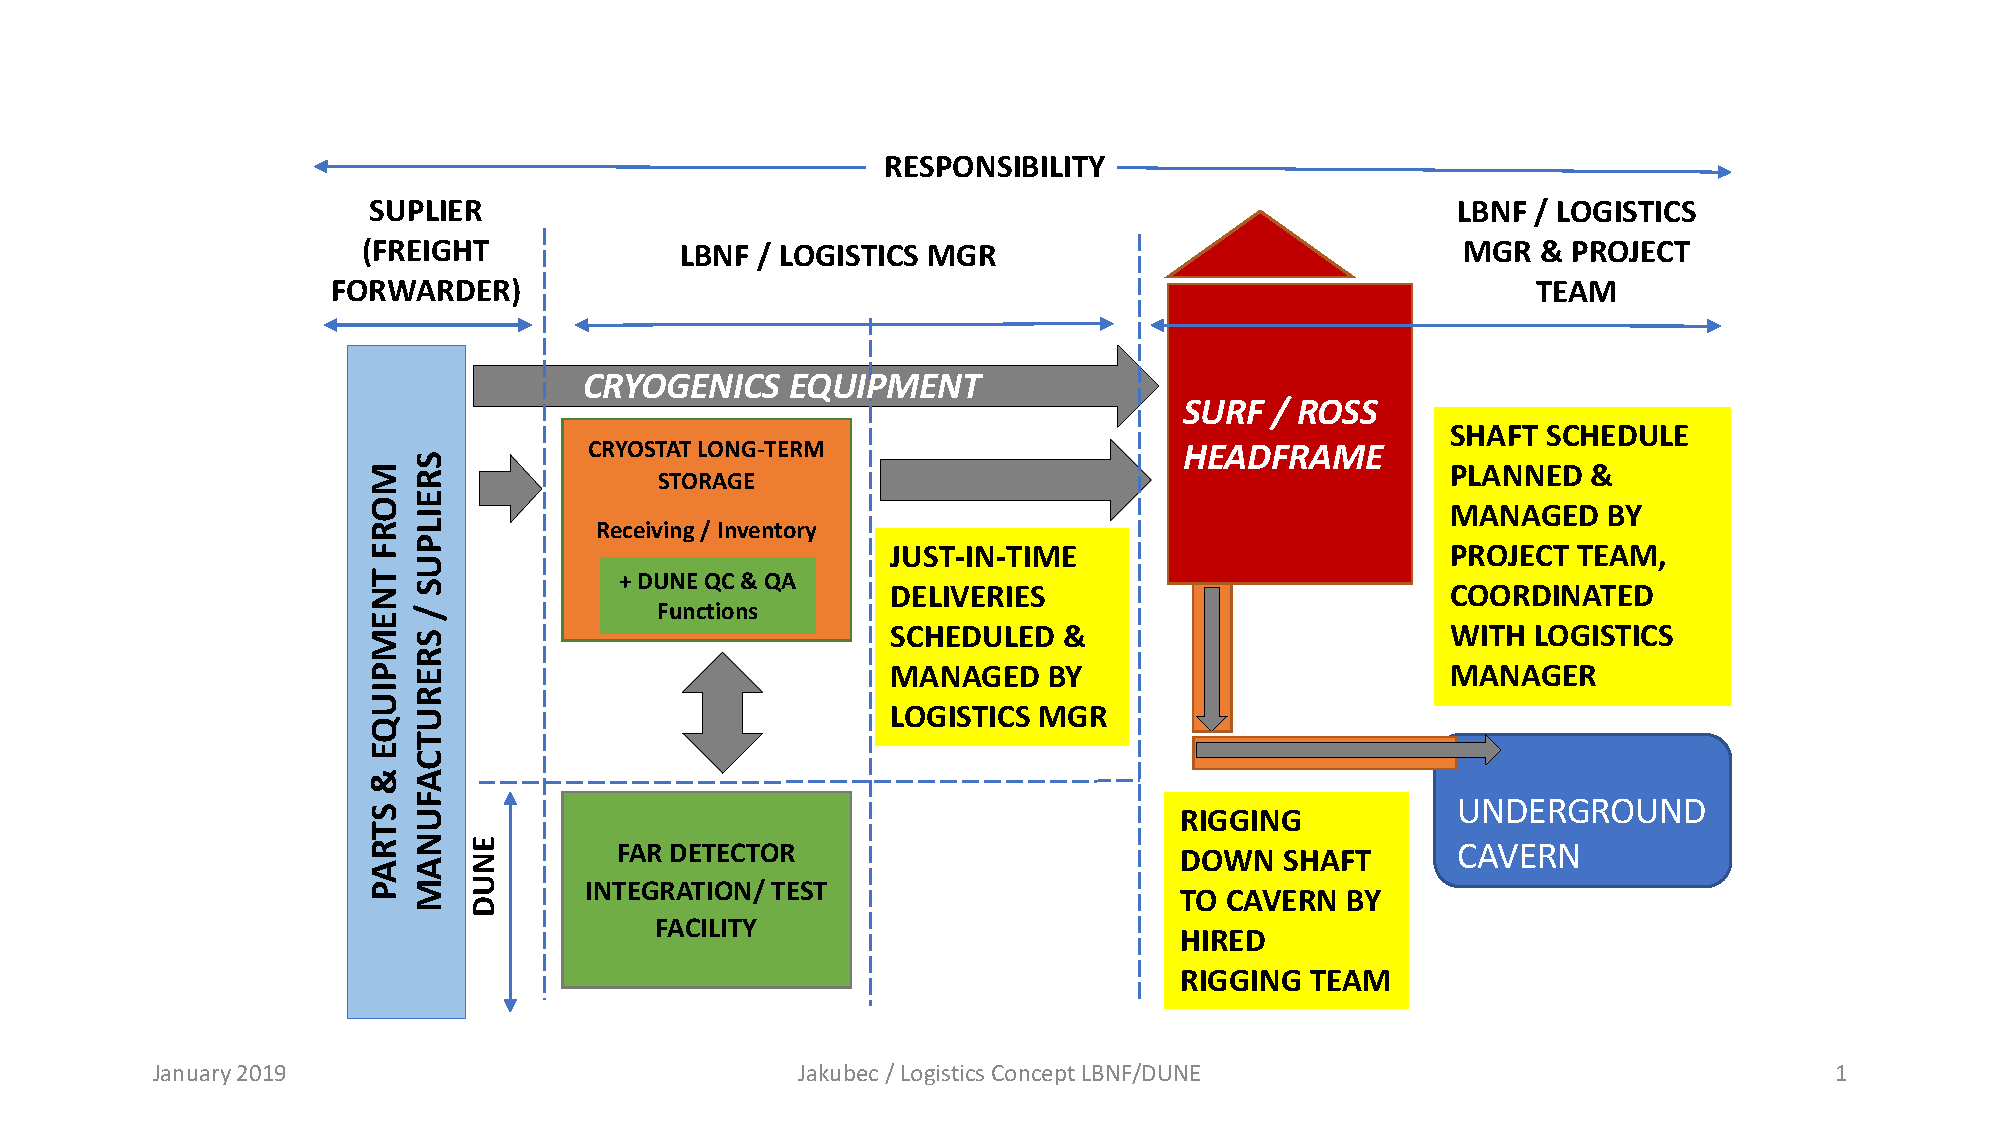
\includegraphics[width=\textwidth]{logistics-material-flow}
\end{dunefigure}


%%%%%%%%%%%%%%%%%%%%%%%%%%%%
\subsection{Logistics Planning}
\label{sec:fdsp-tc-logPln}
The LBNF/DUNE Logistics scope includes overseeing the transportation of the cryostat (steel, foam, and membrane), the cryogenic system, the detector, and all related infrastructure not provided by facilities. The LBNF scope consists of the cryostat and cryogenics system which will not be discussed in detail in this TDR, but as the LBNF material dominates the logistics needs a brief summary here is required. The cryostat steel structure for each cryostat requires bringing roughly 1,800 individual steel pieces underground some which weigh up to 7.5t and about 125t of bolts needed to assemble the steel pieces. The internal structure which includes the foam insulation and the thin stainless steel membrane will require transporting roughly 4,000 boxes each roughly 1.5 $\times$ 3.5 $\times$ 1.2 m$^3$ in dimension. The plan for cryostat installation at present calls for all the components to be warehoused in SD prior to the start of installation. This means that the logistics operation will need roughly 5,000 m$^2$ of warehouse space approximately 2 years prior to the start of DUNE detector installation. By the time DUNE detector components start arriving most the cryostat boxes will have been removed from the warehouse so there will be ample space for the detector and cryogenics components. Additional space may be required if the boxes for the second cryostat arrive before the detector\#1 installation is complete, but several buildings of the required size are available in the area if it is decided expansion is required.


\begin{dunefigure}[Simplified model of the Ross Cage]{fig:fdsp-tc-Cage}
  {Simplified Ross Cage model.}
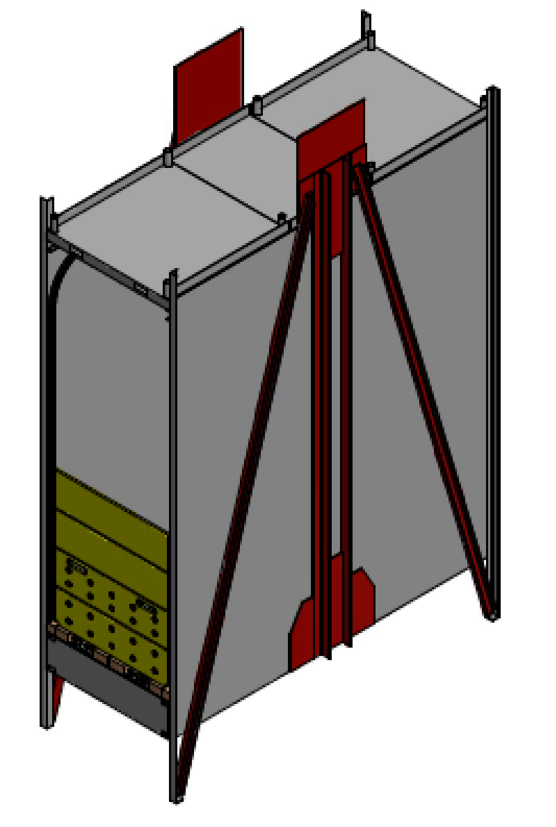
\includegraphics[width=.5\textwidth]{Cage-view}
\end{dunefigure}
%
\begin{dunetable}
[Ross Cage specifications]
{cc}
{tab:table-Ross-Cage}
{Ross Cage Parameters}
Ross Cage Parameters &  
\\ \toprowrule
Inside height &  3.6 m\\ \colhline
Inside depth & 3.7 m \\ \colhline
Inside width & 1.38 m \\
\colhline
Weight limit&  5,897 kg \\
\colhline
Round trip time & 17 min\\ \colhline
\end{dunetable}

All material brought underground must conform to the Sanford Underground Research Facility's (SURF) Facility Access Specification \cite{bib:docdb328}. This document defines the limitations on dimensions and weights for all materials to be transported underground.  The most important limitations which are described in detail in the specification document are related to the Ross shaft and Ross cage. It is possible to bring material down the shaft underneath the cage as a slung load but this is a much slower process and requires careful planning, detailed procedures and review. The DUNE \dword{apa} for example need this special handling as they are too tall to fit in the cage. It is desirable to have most material brought underground inside the cage. Figure \ref{fig:fdsp-tc-Cage} shows an image of the new Ross cage and Table \ref{tab:table-Ross-Cage} summarizes its parameters. As a comparison the round trip travel time for the Ross cage is 17 minutes where most the time needed to load and unload the cage and any slung load will take over an hour round trip as both the loading/unloading and travel times are longer. 

Many other factors need to be considered when planning the DUNE logistics. There is no loading dock at the Ross headframe so all materials will need transported using a flatbed or curtain-sided chassis. The equipment can then be removed with a forklift at SURF. In general the unloading process at SURF needs to be taken into consideration while loading them at the warehouse to avoid difficulties at SURF delivery. The CF-CMGC has to coordinate all the loads through the Ross shaft. To do this DUNE will have to provide 2 weeks advance delivery plan to be incorporated in the overall hoist schedule. DUNE collaborators will not be allowed to ship equipment directly to the Ross Shaft unless it is coordinated by the logistics team. A central inventory system will capture all goods at receipt to the warehouse in South Dakota. DUNE institutions need to provide shipping data and consign cargo accordingly (a shipping manual will be provided by the logistics team) so that the logistics team can monitor the progress. In ProtoDUNE-SP delays in shipping and customs caused up to 3 weeks delay in arrival of some parts which caused significant re-planning of the installation work. In order to prevent this from being a much larger problem in DUNE a minimal one month buffer of materials will be planned. With this the underground work can be planned well in advance knowing all the materials will be available. This will require that sufficient space be available in the warehouse and underground at SURF to house the material buffer. Many small parcels will be arriving at the warehouse from different sources. The warehouse staff will de-consolidate arriving cargo as required and consolidate deliveries to ITF or SURF into larger boxes/crates, as per the ITF or SURF delivery plan, to make efficient use of the truck power and Ross hoist. 


\begin{dunefigure}[Underground space needs during installation setup]{fig:fdsp-tc-setup}
  {Image showing the cavern on end opposite of the detector. During the installation setup phase half the space will be used for the cryostat work and half as storage for the detector infrastructure. The material outside the cavern must be stored in the logistics warehouse.}
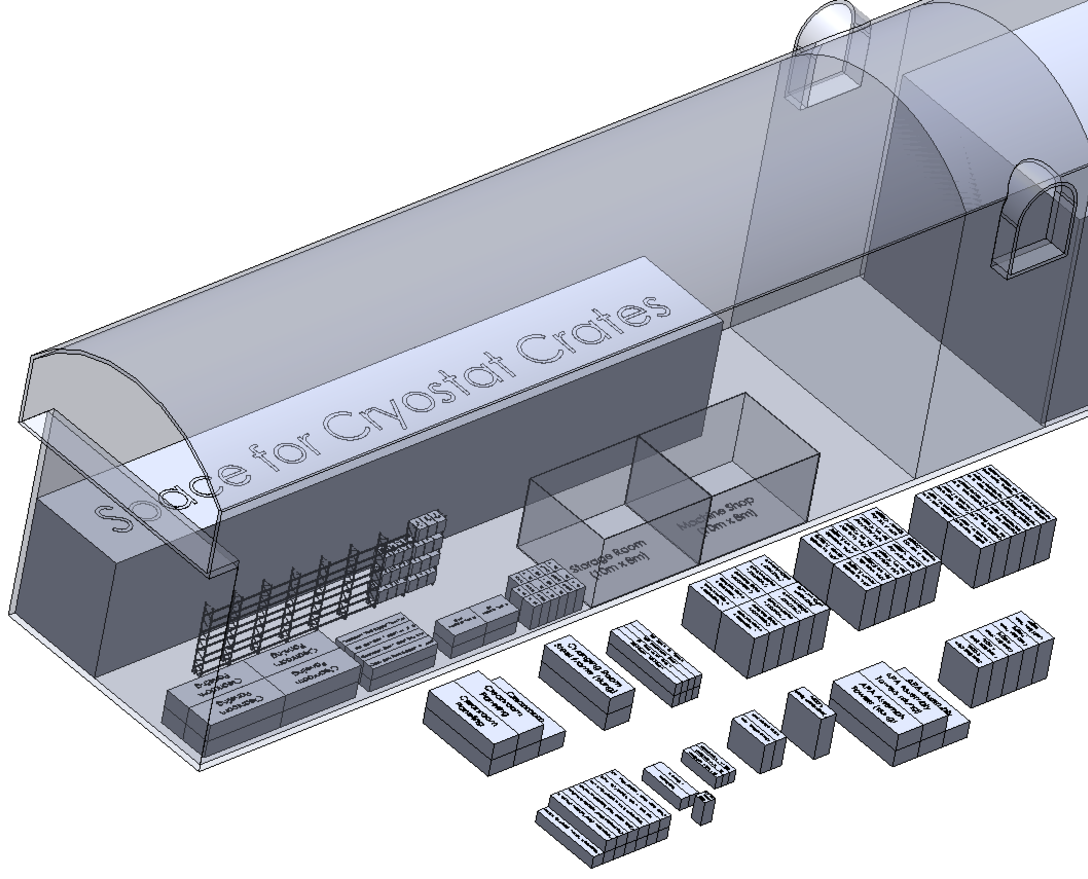
\includegraphics[width=.9\textwidth]{Material-Setup}
\end{dunefigure}
%

In order to understand how much space is needed for storage and how much of the hoist time must be dedicated to DUNE a detailed inventory of all the detector equipment and DUNE infrastructure is needed. The list of all the materials was solicited from all the consortia and technical coordination. The entries in the inventory spreadsheet are organized as "Loads" for the Ross shaft where a load is a crate or set of boxes which will either be transported underground in the hoist or as a slung load.\cite{bib:docdb8426}
%\href{http://docs.dunescience.org/cgi-bin/ShowDocument?docid=8426}{DUNE load Spreadsheet} \cite{bib:docdb8426}

Information captured in the load spreadsheet includes the number of hoist trips, nature of the trip (slung load or cage), the package dimensions, weight and type of package (crate, pallet, box, carton etc.). The load list at present accounts for 1,600 hoist trips and accounts for roughly 2 months of cage time most of which is spread over one year. The installation operation for the single-phase detector will span over 2 years so it is prudent to divide the logistics planning in several phases. The load information is divided into the CUC setup phase, the installation setup phase, and the detector installation phase. In each phase a model was generated to show how much material can be stored underground outside the work area and also how much material needs stored on the surface. These models are used to set the space requirements for the logistics effort on the surface. The phase with the largest amount of material to transport is the detector setup phase and the model of the underground area and the required boxes for surface storage for the first $1/3$\ of the setup is shown in Figure \ref{fig:fdsp-tc-setup}. This represents the first month of installation setup and shows that roughly 1,000 m$^2$\ of warehouse space will be needed for DUNE at this time. In addition to the space needed for receive and ship equipment underground the warehouse will also need space to store up to 150 \dword{apa}. This adds an additional 700 m$^2$\ to the needed warehouse area. 


%%%%%%%%%%%%%%%%%%%%%%%%%%%%
\subsection{Logistics Quality Assurance and Quality Control}
\label{sec:fdsp-tc-log-qaqc}


ProtoDUNE was an extremely useful exercise in general, but only a few conclusions can be drawn related to logistics since shipping to Europe will be different than shipping to South Dakota and the CERN receiving and transport divisions will not be used for DUNE. The most important lessons learned from ProtoDUNE related to logistics are listed below.
\begin{enumerate}
\item Lack of a central inventory system made it impossible to track shipments.
\item Delays in shipping meant that the installation work could not be planned and parts were installed as they arrived. 
\end{enumerate}

To address these issues an inventory system will be implemented at the logistics warehouse facility and a minimum one month material buffer will be required from the consortia in South Dakota.

It is not foreseen to do component testing in the warehouse so the scope of the quality control work there is limited. But there will have to be QA/QC component at receiving. One critical QC check that will be performed at the logistics facility is a check to ensure that all materials to be shipped to the Ross headframe will fit in the cage. Additionally if a slung load is needed the facility will confirm that the necessary procedures are in place and approved before any material is transported to SURF. The other primary QC function performed at the logistic facility is the inventory of all shipments described below.

The nature of this project with the "contribution in kind" model makes the logistics and inventory control as well as gathering of the relevant "construction" data extremely complex. Therefore, the logistics (inventory) control and scientific data collection need to be controlled by independent systems. 
The logistics supply chain will be controlled by the contributors freight forwarding system till arrival at the (yet to be defined/established) "South Dakota Warehouse Facility" (SDWF).  SDWF will be the ultimate "Point of Capture" for all LBNF/DUNE parts/equipment with the possible exemption the Cryogenic system as per the contractual requirements.
The inventory process at the SDWF, the ITF and the SURF receiving at Ross Shaft will be controlled by one integrated commercial Warehouse Management System (WMS), There will be need for some workflow functionality at ITF pre-assembly.
The Warehouse Management System (WMS/inventory) will provide basic receiving, inventory and shipping status information for all parts/equipment delivered to SDWF. That will include pre-assembled equipment that will enter as "new" parts from ITF as created by the work flow.
The QC/QA, manufacturing and other relevant data required/needed/desired by the DUNE collaboration will be stored in a separate yet to be defined and developed DUNE construction database. 
This DUNE construction database is independent of the WMS system and the relevant contributing consortia have the responsibility to transfer the required data prior to shipment from supplier to the DUNE construction database (DCDB).  The WMS database will provide the relevant/required/desired logistics data to the DCDB. The form of data transfer is yet to be determined.
All QC/QA, test and other relevant manufacturing data will be direct input into DCDB and will be the responsibility of the different contributing consortia (DUNE). DUNE will have to provide a QC/QA process for all parts/equipment received at the warehouse after being inventoried. That QC/QA data must be transfer directly to DCDB by DUNE. 
The DCDB will be an integral part of the logistic, assembly and QC/QA system. It will need to provide the ITF shipping (supply) and assembly reports as well as create the new "equipment" denomination for the WMS to register.  The DCDB will document the ITF subassembly process in its entirety (workflow).
The "new" sub-assembled items will be inventoried in WMS as new items during the warehouse receiving process.
The SURF installation management team will be responsible for providing a shipping (supply) report to the warehouse for scheduling of parts/equipment shipments to SURF.
The shipments from SDWF to SURF will be inventoried as received at SURF in WMS.
The DUNE installation team has to transfer the relevant QC/QA, test and installed status data to the DCDB directly.
To capture all relevant construction and logistics data on parts/equipment the following process for the logistics information is foreseen:

\begin{itemize}
\item The consortia must enter data related to any shipment to the SDWF in the WMS.
\item The shipments from SDWF to SURF will be inventoried as received at SURF in the WMS.
\item The SURF installation management team will be responsible for providing a shipping (supply) report to the warehouse for scheduling of parts/equipment shipments to SURF 2 weeks in advance of any shipment.
\end{itemize}







%%%%%%%%%%%%%%%%%%%%%%%%%%%%
\subsection{Logistics Safety}
\label{sec:fdsp-tc-log-safety}

The LBNF/DUNE Logistics Facility is operated by SDSD (South Dakota Systems Division) as a Fermilab Facility, but because of the international presence, we also follow CERN HSE, Fermilab ES\&H and SURF ES\&H regulations.  Work is in progress to combine all of this into a coherent list of codes and requirements to follow. The \dword{dune} Project ES\&H Coordinator has overall ES\&H oversight responsibility for the DUNE Project.  This person coordinates any activities and facilitates the resolution of any issues that cut across various Divisions and institutions. It is subject to the requirements of the DOE Workers Safety and Health Program, Title 10, Code Federal Regulations (CRF) Part 851 (10 CFR 851). These requirements are promulgated through the Fermilab Directors Policy Manual and Fermilab ES\&H manual (FESHM) which align with the SURF ES\&H Manual. 
Using the NOvA Far Detector Lab as a guideline for remote facilities there are several other key documents that guide the Logistics Center Safety Program.  The Building Safety Plan combines all of the building specific documents in a single folder:

\begin{enumerate}
\item	Fire Safety and Building Emergency Evacuation Plan- Fire evacuation plan, fire safety plan and lockdown plans, site plan
\item	Hazard Analysis- Describes all the typical hazards and their mediation including procedures 
\item	SDS- Safety Data Sheets
\item	Respiratory Plan- As required due to chemical or ODH hazards
\item	Training Program- Covers certifications required and  training records
\end{enumerate}

The current Technical Coordination facilities management plan has a joint safety officer used between the ITF and Logistics facility. This safety officer would facilitate training, write Hazard Analysis documents, run the weekly safety meetings, and keep documentation records on materials handling equipment and personnel. 


%%%%%%%%%%%%%%%%%%%%%%%%%%%%
\subsection{Cost, Schedule and Risk Analysis}
\label{sec:fdsp-tc-log-cost}



The logistics facility is required approximately 1 year before the warm structure installation begins.  Acceptance for Use and Possession (AUP) for the North cavern and CUC is October 2022.  Extra storage is also needed for APA pairs for integration, CUC infrastructure and equipment all begin showing up in  South Dakota the summer of 2021. Figure 1.20 shows the overview of the schedule of main activities for Detector 1.

%\fixme{use templates from cost-risk-sched.tex file. Anne}
